\section{Vector-Valued Functions}\label{sec:vvf}

% todo state how this compares with 10.2 & 10.3

We are very familiar with \textbf{real valued functions}, that is, functions whose output is a real number. This section introduces \textbf{vector-valued functions} --- functions whose output is a vector.

\begin{definition}[Vector-Valued Functions]\label{def:vvf}
A \textbf{vector-valued function} is a function of the form 
\[\vec r(t) =\bracket{\, f(t),g(t)\,}\quad \text{or}\quad \vec r(t) =\bracket{\,f(t),g(t),h(t)\,},\]
where $f$, $g$ and $h$ are real valued functions.\bigskip

The \textbf{domain} of $\vec r$ is the set of all values of $t$ for which $\vec r(t)$ is defined. The \textbf{range} of $\vec r$ is the set of all possible output vectors $\vec r(t)$.
\index{vector-valued function!definition}\index{function!vector-valued}
\end{definition}

\subsection{Evaluating and Graphing Vector-Valued Functions}

\mtable[-1in]{Sketching the graph of a vector-valued function.}{fig:vvfintro1}{%
\begin{tikzpicture}[>=stealth]
\begin{axis}[width=1.16\marginparwidth,tick label style={font=\scriptsize},
axis y line=middle,axis x line=middle,name=myplot,xtick={1,2,3,4,5},
ytick={-3,-2,-1,1,2,3},ymin=-3.5,ymax=3.5,xmin=-.5,xmax=5.5]
\draw [->,thick,draw={\colortwo}] (axis cs: 0,0) -- (axis cs:4,1)
 node [black,pos=.5,above] {\scriptsize $\vec r(-2)$};
\end{axis}
\node [right] at (myplot.right of origin) {\scriptsize $x$};
\node [above] at (myplot.above origin) {\scriptsize $y$};
\end{tikzpicture}
\\(a)\\
\begin{tikzpicture}[>=stealth]
\begin{axis}[width=1.16\marginparwidth,tick label style={font=\scriptsize},
axis y line=middle,axis x line=middle,name=myplot,xtick={1,2,3,4,5},
ytick={-3,-2,-1,1,2,3},ymin=-3.5,ymax=3.5,xmin=-.5,xmax=5.5]
\addplot [thick,draw={\colorone}, smooth,domain=-2.5:2.5] ({x^2},{x^2+x-1});
\draw [->,thick,] (axis cs:1,-1)--(axis cs: 0.9025,-1.0475);
\draw [->,thick,draw={\colortwo}] (axis cs: 0,0) -- (axis cs:4,1)
 node[black,pos=.5,above] {\scriptsize $\vec r(-2)$};
\end{axis}
\node [right] at (myplot.right of origin) {\scriptsize $x$};
\node [above] at (myplot.above origin) {\scriptsize $y$};
\end{tikzpicture}
\\(b)}

Evaluating a vector-valued function at a specific value of $t$ is straightforward; simply evaluate each component function at that value of $t$. For instance, if $\vec r(t) =\bracket{t^2,t^2+t-1}$, then $\vec r(-2) =\bracket{4,1}$. We can sketch this vector, as is done in \autoref{fig:vvfintro1}(a). Plotting lots of vectors is cumbersome, though, so generally we do not sketch the whole vector but just the terminal point. The \textbf{graph} of a vector-valued function is the set of all terminal points of $\vec r(t)$, where the initial point of each vector is always the origin. In \autoref{fig:vvfintro1}(b) we sketch the graph of $\vec r$\,; we can indicate individual points on the graph with their respective vector, as shown.
\index{vector-valued function!graphing}

Vector-valued functions are closely related to parametric equations. While in both methods we plot points $\bigl(x(t), y(t)\bigr)$ or $\bigl(x(t),y(t),z(t)\bigr)$ to produce a graph, in the context of vector-valued functions each such point represents a vector. The implications of this will be more fully realized in the next section as we apply calculus ideas to these functions.

\youtubeVideo{Djtttm0C7zA}{Domain of a Vector-Valued Function}

\mtable[-\baselineskip]{Sketching the vector-valued function of \autoref{ex_vvf1}.}{fig:vvf1}{%
\begin{tabular}{ c c c }
	$t$ & $t^3-t$ & $\ds \frac{1}{t^2+1}$ \\[6pt] \midrule
	$-2$&$-6$& 1/5\\  $-1$&0&1/2\\ 0&0&1\\ 1&0&1/2 \\ 2&6&1/5		
\end{tabular}
\\(a)\\[10pt]
\begin{tikzpicture}[>=stealth]
\begin{axis}[width=1.16\marginparwidth,tick label style={font=\scriptsize},
axis y line=middle,axis x line=middle,name=myplot,xtick={-6,-4,-2,2,4,6},
ymin=-.1,ymax=1.1,xmin=-7,xmax=7]
\addplot [thick,draw={\colorone}, smooth,domain=-2:2] ({x^3-x},{1/(x^2+1)});
\filldraw [black] (axis cs: -6,.2) circle (1.5pt);
\filldraw [black] (axis cs: 6,.2) circle (1.5pt);
\filldraw [black] (axis cs: 0,.5) circle (1.5pt);
\filldraw [black] (axis cs: 0.,1) circle (1.5pt);
\draw [->,thick,draw={\colortwo}] (axis cs:0,0)--(axis cs: 0,.5)
 node [,black,pos=.4,rotate=90,above] {\scriptsize $\vec r(-1)$};
\draw [->,thick,draw={\colortwo}] (axis cs:0,0)--(axis cs: 6,.2)
 node [black,pos=.4,above] {\scriptsize $\vec r(2)$};
\end{axis}
\node [right] at (myplot.right of origin) {\scriptsize $x$};
\node [above] at (myplot.above origin) {\scriptsize $y$};
\end{tikzpicture}
\\(b)}

\begin{example}[Graphing vector-valued functions]\label{ex_vvf1}
Graph $\ds \vec r(t) =\bracket{t^3-t, \frac{1}{t^2+1}}$, for $-2\leq t\leq 2$. Sketch $\vec r(-1)$ and $\vec r(2)$.
\solution
We start by making a table of $t$, $x$ and $y$ values as shown in \autoref{fig:vvf1}(a). Plotting these points gives an indication of what the graph looks like. In \autoref{fig:vvf1}(b), we indicate these points and sketch the full graph. We also highlight $\vec r(-1)$ and $\vec r(2)$ on the graph.
\end{example}

\begin{example}[Graphing vector-valued functions.]\label{ex_vvf2}
Graph $\vec r(t) =\bracket{\cos t,\sin t,t}$ for $0\leq t\leq 4\pi$.
\solution
We can again plot points, but careful consideration of this function is very revealing. Momentarily ignoring the third component, we see the $x$ and $y$ components trace out a circle of radius 1 centered at the origin. Noticing that the $z$ component is $t$, we see that as the graph winds around the $z$-axis, it is also increasing at a constant rate in the positive $z$ direction, forming a spiral. This is graphed in \autoref{fig:vvf2}. In the graph $\vec r(7\pi/4)=\bracket{\frac1{\sqrt2},-\frac1{\sqrt2},\frac{7\pi}4}%\approx \bracket{0.707,-0.707,5.498}
$ is highlighted to help us understand the graph.
\end{example}

\mtable[-.5in]{Viewing a vector-valued function, and its value at one point.}{fig:vvf2}{\myincludeasythree{width=\marginparwidth,
3Droll=1.5110919487882861,
3Dortho=0.0044999998062849045,
3Dc2c=0.6482614874839783 0.682218074798584 0.338135302066803,
3Dcoo=1.5296688079833984 -8.776086807250977 69.70178985595703,
3Droo=399.99999354879714}{width=\marginparwidth}{figures/figvvf2_3D}}

%\subsection{Algebra of Vector-Valued Functions}
%
%\begin{definition}[Operations on Vector-Valued Functions]\label{def:vvf_algebra}
%Let $\vec r_1(t)=\bracket{f_1(t),g_1(t)}$ and $\vec r_2(t)=\bracket{f_2(t),g_2(t)}$ be vector-valued functions in $\mathbb{R}^2$ and let $c$ be a scalar. Then:
%\begin{enumerate}
%	\item $\vec r_1(t) \pm \vec r_2(t) =\bracket{\, f_1(t)\pm f_2(t),g_1(t)\pm g_2(t)\,}$.
%	\item	$c\vec r_1(t) =\bracket{\, cf_1(t),cg_1(t)\,}$.
%\end{enumerate}
%A similar definition holds for vector-valued functions in $\mathbb{R}^3$.
%\index{vector-valued function!algebra of}
%\end{definition}
%
%This definition states that we add, subtract and scale vector-valued functions component-wise. Combining vector-valued functions in this way can be very useful (as well as create interesting graphs).

\begin{example}[Adding and scaling vector-valued functions.]\label{ex_vvf3}
Let $\vec r_1(t) =\bracket{\,0.2t,0.3t\,}$, $\vec r_2(t) =\bracket{\,\cos t,\sin t\,}$ and $\vec r(t) = \vec r_1(t)+\vec r_2(t)$. Graph $\vec r_1(t)$, $\vec r_2(t)$, $\vec r(t)$ and $5\vec r(t)$ on $-10\leq t\leq10$.
\solution
We can graph $\vec r_1$ and $\vec r_2$ easily by plotting points (or just using technology). Let's think about each for a moment to better understand how vector-valued functions work.

We can rewrite $\vec r_1(t) =\bracket{\, 0.2t,0.3t\,}$ as $ \vec r_1(t) = t\bracket{0.2,0.3}$. That is, the function $\vec r_1$ scales the vector $\bracket{0.2,0.3}$ by $t$. This scaling of a vector produces a line in the direction of $\bracket{0.2,0.3}$.

We are familiar with $\vec r_2(t) =\bracket{\, \cos t,\sin t\,}$; it traces out a circle, centered at the origin, of radius 1. \autoref{fig:vvf3}(a) graphs $\vec r_1(t)$ and $\vec r_2(t)$.

\mtable{Graphing the functions in \autoref{ex_vvf3}.}{fig:vvf3}{%
\begin{tikzpicture}[>=stealth]
\begin{axis}[width=1.16\marginparwidth,tick label style={font=\scriptsize},
axis y line=middle,axis x line=middle,name=myplot,
ymin=-4.1,ymax=4.1,xmin=-4.9,xmax=4.9]
\addplot [thick,draw={\colorone}, smooth,domain=-10:10] ({.2*x},{.3*x});
\draw[thick,draw={\colorone},smooth](axis cs:0,0)circle(1);
%\addplot [thick,draw={\colorone}, smooth,domain=0:360] ({cos(x)},{sin(x)});
\end{axis}
\node [right] at (myplot.right of origin) {\scriptsize $x$};
\node [above] at (myplot.above origin) {\scriptsize $y$};
\end{tikzpicture}
\\(a)\\[10pt]
\begin{tikzpicture}[>=stealth]
\begin{axis}[width=1.16\marginparwidth,tick label style={font=\scriptsize},
axis y line=middle,axis x line=middle,name=myplot,
ymin=-4.1,ymax=4.1,xmin=-4.9,xmax=4.9]
\addplot [thick,draw={\colorone}, smooth,domain=-10:10,samples=60]
 ({.2*x+cos(deg(x))},{.3*x+sin(deg(x))});
\end{axis}
\node [right] at (myplot.right of origin) {\scriptsize $x$};
\node [above] at (myplot.above origin) {\scriptsize $y$};
\end{tikzpicture}
\\(b)\\[10pt]
\begin{tikzpicture}[>=stealth]
\begin{axis}[width=1.16\marginparwidth,tick label style={font=\scriptsize},
axis y line=middle,axis x line=middle,name=myplot,xtick={-20,-10,10,20},
ymin=-20.5,ymax=20.5,xmin=-24.5,xmax=24.5]
\addplot [thick,draw={\colorone}, smooth,domain=-10:10,samples=60]
 ({.2*x+cos(deg(x))},{.3*x+sin(deg(x))});
\addplot [thick,draw={\colorone}, smooth,domain=-10:10,samples=60]
 ({x+5*cos(deg(x))},{1.5*x+5*sin(deg(x))});
\end{axis}
\node [right] at (myplot.right of origin) {\scriptsize $x$};
\node [above] at (myplot.above origin) {\scriptsize $y$};
\end{tikzpicture}
\\(c)}

Adding $\vec r_1(t)$ to $\vec r_2(t)$ produces $\vec r(t) =\bracket{\,\cos t + 0.2t,\sin t+0.3t\,}$, graphed in \autoref{fig:vvf3}(b). The linear movement of the line combines with the circle to create loops that move in the direction of $\bracket{0.2,0.3}$.  (We encourage the reader to experiment by changing $\vec r_1(t)$ to $\bracket{2t,3t}$, etc., and observe the effects on the loops.)

Multiplying $\vec r(t)$ by 5 scales the function by 5, producing
\[5\vec r(t) =\bracket{5\cos t+t,5\sin t+\frac32t},\]
which is graphed in \autoref{fig:vvf3}(c) along with $\vec r(t)$. The new function is ``5 times bigger'' than $\vec r(t)$. Note how the graph of $5\vec r(t)$ in (c) looks identical to the graph of $\vec r(t)$ in $(b)$. This is due to the fact that the $x$ and $y$ bounds of the plot in $(c)$ are exactly 5 times larger than the bounds in (b).
\end{example}

\begin{example}[Adding and scaling vector-valued functions.]\label{ex_vvf4}
A \textbf{cycloid} is a graph traced by a point $p$ on a rolling circle, as shown in \autoref{fig:vvf4}. Find an equation describing the cycloid, where the circle has radius 1.
\index{cycloid}
{\centering
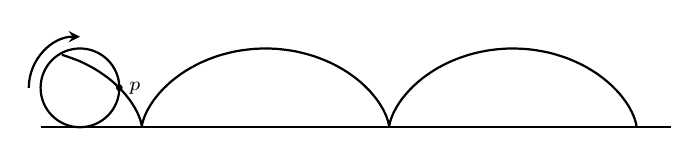
\begin{tikzpicture}[>=stealth,scale=.5]
\draw [thick] (0,1) circle (1);
\filldraw (1,1) circle (2pt) node [right] {\scriptsize $p$};
\draw [draw={\colorone},thick,domain=-1:14,smooth,samples=60]
 plot ({cos(\x r)+\x},{-sin(\x r)+1});
\draw [thick] (-1,0) -- (15,0);
\draw [thick,->] (-1.3,1) arc (180:90:1.3);
\draw [thick,white] (0,2.5) -- (1,2.5);
\end{tikzpicture}
\captionsetup{type=figure}
\caption{Tracing a cycloid.}\label{fig:vvf4}
}% end centering
\solution
This problem is not very difficult if we approach it in a clever way. We start by letting $\vec p(t)$ describe the position of the point $p$ on the circle, where the circle is centered at the origin and only rotates clockwise (i.e., it  does not roll). This is relatively simple given our previous experiences with parametric equations; $\vec p(t) =\bracket{\cos t, -\sin t}$. 

We now want the circle to roll. We represent this by letting $\vec c(t)$ represent the location of the center of the circle. It should be clear that the $y$ component of $\vec c(t)$ should be 1; the center of the circle is always going to be 1 if it rolls on a horizontal surface.

%% to do how does this differ from the previous figure?
%\mtable{The cycloid in \autoref{ex_vvf4}.}{fig:vvfa}{\begin{tikzpicture}[>=stealth]
%\begin{axis}[width=1.16\marginparwidth,tick label style={font=\scriptsize},
%axis y line=middle,axis x line=middle,name=myplot,
%ymin=-.1,ymax=14,xmin=-.5,xmax=16]
%\addplot [thick,draw={\colorone}, smooth,domain=-1:16,samples=60]
% ({cos(deg(x))+x},{-sin(deg(x))+1});
%\end{axis}
%\node [right] at (myplot.right of origin) {\scriptsize $x$};
%\node [above] at (myplot.above origin) {\scriptsize $y$};
%\end{tikzpicture}}

The $x$ component of $\vec c(t)$ is a linear function of $t$: $f(t) = mt$ for some scalar $m$. When $t=0$, $f(t) = 0$ (the circle starts centered on the $y$-axis). When $t=2\pi$, the circle has made one complete revolution, traveling a distance equal to its circumference, which is also $2\pi$. This gives us a point on our line $f(t) = mt$, the point $(2\pi, 2\pi)$. It should be clear that $m=1$ and $f(t) = t$. So $\vec c(t) =\bracket{t, 1}$. 

We now combine $\vec p$ and $\vec c$ together to form the equation of the cycloid: $\vec r(t) = \vec p(t) + \vec c(t) =\bracket{\cos t+ t,-\sin t+1}$, which
matches the graph in \autoref{fig:vvf4}.
% is graphed in \autoref{fig:vvfa}.
\end{example}

\subsection{Displacement}

A vector-valued function $\vec r(t)$ is often used to describe the position of a moving object at time $t$. At $t=t_0$, the object is at $\vec r(t_0)$; at $t=t_1$, the object is at $\vec r(t_1)$. Knowing the locations $\vec r(t_0)$ and $\vec r(t_1)$ give no indication of the path taken between them, but often we only care about the difference of the locations, $\vec r(t_1)-\vec r(t_0)$, the \textbf{displacement}.\index{displacement}\index{vector-valued function!displacement}

\begin{definition}[Displacement]\label{def:displacement}
Let $\vec r(t)$ be a vector-valued function and let $t_0<t_1$ be values in the domain. The \textbf{displacement} $\vec d$ of $\vec r$, from $t=t_0$ to $t=t_1$, is \[\vec d=\vec r(t_1)-\vec r(t_0).\]
\end{definition}

When the displacement vector is drawn with initial point at $\vec r(t_0)$, its terminal point is $\vec r(t_1)$. We think of it as the vector which points from a starting position to an ending position.

\begin{example}[Finding and graphing displacement vectors]\label{ex_vvf5}
Let $\vec r(t) =\bracket{\cos (\frac{\pi}{2}t),\sin (\frac{\pi}2 t)}$. Graph $\vec r(t)$ on $-1\leq t\leq 1$, and find the displacement of $\vec r(t)$ on this interval.
\solution
The function $\vec r(t)$ traces out the unit circle, though at a different rate than the ``usual'' $\bracket{\cos t,\sin t}$ parameterization. At $t_0=-1$, we have $\vec r(t_0) =\bracket{0,-1}$; at $t_1=1$, we have $\vec r(t_1) =\bracket{0,1}$. The displacement of $\vec r(t)$ on $[-1,1]$ is thus $\vec d =\bracket{0,1}-\bracket{0,-1}=\bracket{0,2}.$

\mtable{Graphing the displacement of a position function in \autoref{ex_vvf5}.}{fig:vvf5}{\begin{tikzpicture}[>=stealth]
\begin{axis}[width=1.16\marginparwidth,tick label style={font=\scriptsize},
axis y line=middle,axis x line=middle,name=myplot,ytick={-1,1},
ymin=-1.1,ymax=1.1,xmin=-1.32,xmax=1.32]
\addplot [thick,draw={\colorone}, smooth,domain=-90:90,samples=20] ({cos(x)},{sin(x)});
\draw [thick,->,draw={\colortwo}] (axis cs: 0,-1) -- (axis cs:0,1)
 node [left,pos=.7,black]{\scriptsize $\vec d$};
\end{axis}
\node [right] at (myplot.right of origin) {\scriptsize $x$};
\node [above] at (myplot.above origin) {\scriptsize $y$};
\end{tikzpicture}}

A graph of $\vec r(t)$ on $[-1,1]$ is given in \autoref{fig:vvf5}, along with the displacement vector $\vec d$ on this interval.
\end{example}

Measuring displacement makes us contemplate related, yet very different, concepts. Considering the semi-circular path the object in \autoref{ex_vvf5} took, we can quickly verify that the object ended up a distance of 2 units from its initial location. That is, we can compute $\vnorm{d} = 2$. However, measuring \emph{distance from the starting point} is different from measuring \emph{distance traveled}. Being a semi-circle, we can measure the distance traveled by this object as $\pi%\approx 3.14
$ units. Knowing \emph{distance from the starting point} allows us to compute \textbf{average rate of change.}

\begin{definition}[Average Rate of Change]\label{def:av_rate_of_change_vect}
Let $\vec r(t)$ be a vector-valued function, where each of its component functions is continuous on its domain, and let $t_0<t_1$. The \textbf{average rate of change} of $\vec r(t)$ on $[t_0,t_1]$ is
\index{average rate of change}\index{vector-valued function!average rate of change}
\[\text{average rate of change} = \frac{\vec r(t_1) - \vec r(t_0)}{t_1-t_0}.\]
\end{definition}

\begin{example}[Average rate of change]\label{ex_vvf6}
Let $\vec r(t) =\bracket{\cos(\frac{\pi}2t),\sin(\frac{\pi}2t)}$ as in \autoref{ex_vvf5}. Find the average rate of change of $\vec r(t)$ on $[-1,1]$ and on $[-1,5]$.
\solution
We computed in \autoref{ex_vvf5} that the displacement of $\vec r(t)$ on $[-1,1]$ was $\vec d =\bracket{0,2}$. Thus the average rate of change of $\vec r(t)$ on $[-1,1]$ is:
\[\frac{\vec r(1) -\vec r(-1)}{1-(-1)} = \frac{\bracket{0,2}}{2} =\bracket{0,1}.\]
We interpret this as follows: the object followed a semi-circular path, meaning it moved towards the right then moved back to the left, while climbing slowly, then quickly, then slowly again. \emph{On average}, however, it progressed straight up at a constant rate of $\bracket{0,1}$ per unit of time.

We can quickly see that the displacement on $[-1,5]$ is the same as on $[-1,1]$, so $\vec d =\bracket{0,2}$. The average rate of change is different, though:
\[\frac{\vec r(5)-\vec r(-1)}{5-(-1)} = \frac{\bracket{0,2}}{6} =\bracket{0,1/3}.\]
As it took ``3 times as long'' to arrive at the same place, this average rate of change on $[-1,5]$ is $1/3$ the average rate of change on $[-1,1]$.
\end{example}

We considered average rates of change in Sections \ref{sec:limit_intro} and \ref{sec:derivative} as we studied limits and derivatives. The same is true here; in the following section we apply calculus concepts to vector-valued functions as we find limits, derivatives, and integrals. Understanding the average rate of change will give us an understanding of the derivative; displacement gives us one application of integration.

\printexercises{exercises/11-01-exercises}
